\chapter{Diseño}
\thispagestyle{empty}

\section{Descripción del capítulo} \label{sec:\thesection}
En este capítulo se analizarán los requerimientos presentados en la sección \ref{sec:1.5} del capítulo 1 con el objetivo de determinar qué se planea hacer para cumplirlos.

\section{REQ-01} \label{sec:\thesection}
Para cumplir este requerimiento se debe contar con herramientas de software que permita el manejo de: freno, leds indicadores, fin de carrera, dipswitch, encoders AB de disco y motor, motor y DMX. Además, como la placa de control no cuenta con un puerto de debug es necesario tener algún canal de comunicación alternativo, como un puerto serie por software. También será necesario temporizar ciertas partes del programa, por lo que se deberá poder manejar un timer.\\
El microcontrolador utilizado en la placa de control es el Atmega328p, y cuenta con periféricos para manejar todas las entradas y salidas del sistema por lo que es una buena elección para el proyecto. El único inconveniente que presenta es que es un microcontrolador de 8 bits con relativamente baja memoria y sin optimizaciones para operaciones de punto flotante. 

En sistemas embebidos, la manera de manejar el hardware del microcontrolador, entre otras cosas, es a través de librerías. Estas son un conjunto de funciones o procedimientos externos a la aplicación a desarrollar que le permiten al usuario manejar ciertos aspectos del sistema de forma más fácil.\\
Una opción sería utilizar librerías ya desarrolladas, entre las cuales se destacan las de Arduino. Arduino, una plataforma de programación de sistemas embebidos muy popular, utiliza en sus placas microcontroladores de marca Atmel. En particular, el \textit{Arduino UNO} utiliza el Atmega328p, por lo que existen funciones provistas por Arduino para el manejo de los periféricos del microcontrolador que se utiliza en el proyecto. \\
La otra opción sería hacer librerías a medida para el proyecto, desarrollando las funciones necesarias para el manejo de los periféricos que se necesiten para que se comporten exactamente como uno desea.\\
En la tabla \ref{table:2.1} se presenta una comparación entre ambas opciones.

El mayor problema con las librerías de Arduino es que para que cuadren en proyectos grandes como estos requieren modificaciones, y las funciones provistas deben ser analizadas para verificar que no se usen elementos como delays bloqueantes ni operaciones de punto flotante indiscriminadamente, ya que deterioran el rendimiento. \\
Como el objetivo es hacer que el sistema sea lo más confiable posible, y teniendo en cuenta que el tiempo de desarrollo no es un factor crítico, \textbf{se desarrollarán librerías propias para manejar los periféricos}.\\

\begin{table}[!ht]
	\begin{center}
		\begin{tabular}{|c|l|l|}
			\hline
			\textbf{} & \textbf{Arduino} & \textbf{Propia} \\
			\hline \hline
			Pros & - Listas para usar & - Bajo uso de recursos \\
			& - Altamente testeadas  & - Confiabilidad \\
			& - Mantenidas por una comunidad & - Predictibilidad \\
			\hline
			Cons & - Genéricas (poco optimizadas) & - Tiempo de desarrollo alto por defecto \\
			& - Necesitan modificaciones para ser útiles & - Investigación y estudio \\
			& - Requieren análisis &   \\
			\hline
		\end{tabular}
	\end{center}
	\caption{Comparación entre el uso de librerías de Arduino vs el desarrollo de unas propias}
	\label{table:\thetable}
\end{table}

\section{REQ-02} \label{sec:\thesection}
\subsection{Esquema de control}
Para cumplir con este requerimiento la carga se debe mover en respuesta a una referencia de posición y otra de velocidad indicadas por una consola DMX. Para esto se utilizará el esquema de control mostrado en la figura \ref{fig:2.1}, siendo: p la posición, v la velocidad,  Cp el controlador de posición, Cv el de velocidad, \(\varepsilon\)p y \(\varepsilon\)v los errores de posición y velocidad, u la acción de control, G la planta, y rp\_dmx y rv\_dmx las referencias de posición y velocidad dadas por la consola DMX.   \\

\begin{figure}[!ht]
	\centering
	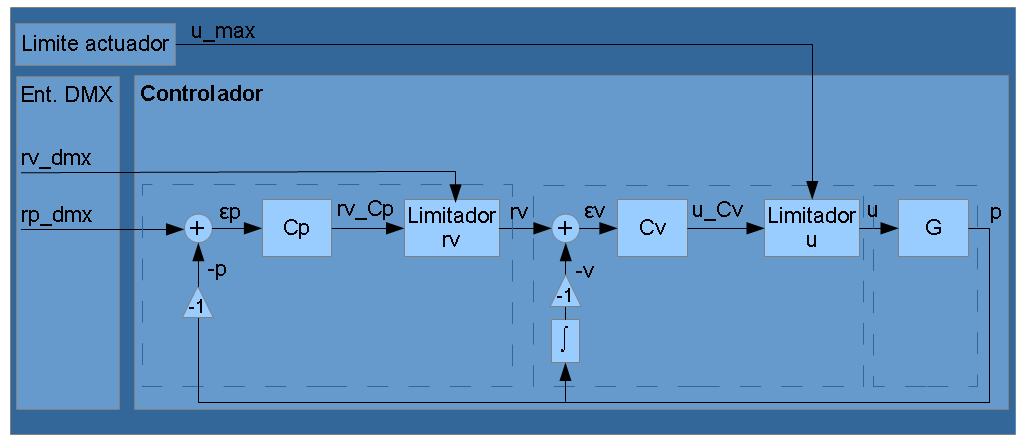
\includegraphics[width=16cm,scale=1]{resources/2_1-diagramaControlador.png}
	\caption{Esquema de control a implementar}
	\label{fig:\thefigure}
\end{figure}

La elección de este esquema fue debido a su simpleza: un controlador de velocidad se encarga de mantener la velocidad igual a la referencia, mientras que uno de posición le indica al de velocidad que debe frenar cuando la posición objetivo está por ser alcanzada. Para evitar que el controlador de posición le indique al de velocidad una referencia mayor a la permitida, se utiliza un limitador en al referencia de velocidad. Similarmente, como la acción de control será el ciclo de trabajo del pwm que mueve al motor, se utiliza un segundo limitador para evitar que el ciclo de trabajo supere el 100 \%.

\subsection{Modelo de la planta}
Para este proyecto la planta será considerada como el conjunto motor-transmisión-carga. Un esquema mecánico de la planta se muestra en la figura \ref{fig:2.2}. Su funcionamiento es el siguiente: parte de la potencia eléctrica que ingresa al motor se transforma a mecánica y se utiliza para mover el piñon que se encuentra conectado al eje del motor. El piñon, a través de una cadena ANSI 25, transfiere su energía a la corona, que hace girar un disco adosado a ella. Este disco, o carrete, contiene en su interior el cable que sostiene a la carga, enrrollandolo o desenrrollandolo para subirla o bajarla. Como la carga del updown puede necesitar ser alimentada y recibir señal de DMX, el cable utilizado contiene en su interior contiene 2 cables con ambas señales.

Ahora, para diseñar el controlador se debe encontrar un modelo matemático de la planta. Una opción es determinar las ecuaciones diferenciales que gobiernan el sistema aplicando la segunda ley de newton, y determinando el modelo matemático de un motor de continua mediante identificación. El problema es que por motivos constructivos del equipo existen muchas piezas que generan roces en diferentes partes del recorrido de la carga, lo que quiere decir que hay una perturbación cuya dinámica es totalmente desconocida y que depende de varios factores, como la distancia y el peso de la carga.\\
Por lo tanto, se abordará el problema con un método más simple: determinar el modelo de todo el conjunto mediante identificación, midiendo la respuesta del sistema ante ciertas entradas. Como el objetivo es que varios updown se comporten lo más parecido posible, se realizarán las pruebas para por lo menos 2 updown. 

\begin{figure}[!ht]
	\centering
	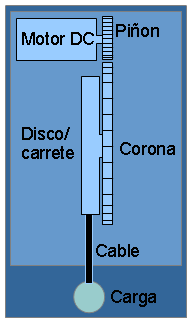
\includegraphics[width=6cm,scale=1]{resources/2_2-modeloMecPlanta.png}
	\caption{Modelo mecánico de la planta}
	\label{fig:\thefigure}
\end{figure}


\subsection{Procedimiento para el diseño de control}
Primero se determinará el período de muestreo y actuación inyectándole un escalón unitario a planta.\\
Luego, se obtendrá el modelo de la planta mediante identificación paramétrica, haciendo uso de un método de estimación de tipo offline (no recursivo).\\
Luego se diseñarán los controladores de posición y velocidad en base al modelo de la planta obtenido\\
Finlamente se validarán los controladores hayados haciendo pruebas directamente sobre el updown.

\subsection{Relación entre cuentas de encoder y distancia}
A medida que el motor gira desenrrolla el cable para subir o bajar la carga. El problema es que dependiendo cuán enrrollada está el cable en el disco un mismo número de cuentas de encoder se puede traducir en distintas distancias recorridas por la carga. Por ejemplo, si el cable está completamente enrollada el radio es mayor, por lo que si giro 360 grados el carrete el largo desenrrollado será uno, mientras que si el cable se encuentra parcialmente desenrrollada el radio es menor, por lo que la distancia descendida en un giro de 360 grados del carrete será otra (menor que la anterior).\\

Para determinar esta relación se harán marcas cada un metro en el cable, tomando como 0 cuando esta está completamente enrrollada, y para cada una se anotará el valor del encoder del motor, que es el que más resolución tiene. Con estos datos se construirá una tabla, se encontrarán varios polinomios que fitteen los datos y se determinará cuál de ellos es el que se implementará en software.

\subsection{Velocidad máxima}
Una tarea a resolver es determinar cuál es la velocidad máxima posible para una carga determinada.\\

Para determinar este valor se medirá la velocidad para una carga de 3Kg en subida aplicando sobre el motor un pwm con ciclo de trabajo de 100\%.

La posición máxima posible queda dada por condiciones de diseño: 4 metros

\section{REQ-03} \label{sec:\thesection}
Los posibles errores detectables que se pueden tener en el equipo son:

\subsection{Corte de correa}
La transmisión de potencia entre el piñon en el eje del motor y la corona en el disco se hace a través de una correa. El problema es que durante las pruebas, la empresa observó que la correa podría cortarse. \\
La manera que tiene el equipo de detectar este error es mediante un segundo encoder AB que mide el giro del disco. Como la relación de vueltas entre el disco y el motor es proporcional, cualquier desviación grande de esta proporcionalidad indica que uno se está moviendo más rápidamente que el otro. Esto podría interpretarse como que la correa fue cortada o que alguno de los encoders dejó de funcionar, 2 errores válidos de hardware.

Para poder detectar estos errores lo primero que se hará es determinar la relación entre las cuentas del encoder del disco y las del motor. Luego verificará en el firmware que esta se cumpla en todo momento, bajo un cierto nivel de error aceptable. En caso de no cumplirse se accionará el freno, se detendrá el equipo completamente y se indicará sobre la existencia del error mediante el led de la placa de control (led interno).

\subsection{Fin de carrera}
La función principal del fin de carrera, un par de pulsadores en la base del equipo, es indicar cuándo el cable que sostiene la carga está completamente enrrollada para determinar la posición 0 o "home" del equipo, dado que este puede estar en cualquier posición al ser encendido.\\
La función secundaria del fin de carrera es detectar posibles eventos indeseados. Por ejemplo, en su punto más bajo la carga se encontrará a 4 metros por debajo del 0 del updown, por lo que podría comenzar a oscilar debido a fuertes vientos o personas que muevan la carga. Por cómo está construido el fin de carrera si la carga oscila más alla de un ángulo de aproximadamente 30 grados el fin de carrera se accionará dando aviso de esto.

Para poder detectar estos errores se verificará que el fin de carrea no sea presionado fuera de la rutina de calibración de (homing). En caso de que sea presionado en estas condiciones se detendrá el equipo, se esperará un tiempo a que la oscilación baje, y intentarán reanudar las operaciones normales. En caso de que el fin de carrera siga presionado se accionará el freno, se detendrá el equipo completamente y se indicará sobre la existencia del error mediante el led de la placa de control (led interno).


\subsection{Pérdida de DMX}
El estándar DMX establece que el tiempo máximo entre un paquete de datos y otro, tiempo de IDLE o MTBP (ver tabla \ref{table:1.1}), es de 1 segundo. Esto quiere decir que si por 1 segundo no me llegaron nuevos datos se considera que se perdió la comunicación con el dispositivo DMX.

Para detectar la pérdida de señal de DMX se verificará constantemente que el último paquete haya llegado hace menos de 1 segundo. En caso de no cumplirse se asumirá que las referencias de posición y velocidad son 0 (equipo parado). Además, por una convención en equipos DMX, se indicará mediante el led en el dipswitch (led externo) cuándo el equipo recibe correctamente la señal de DMX y cuándo no, encendiendolo y apagándolo rápidamente en el primer caso y lentamente en el segundo.


\section{REQ-04} \label{sec:\thesection}
El propósito del dipswitch en el equipo es poder seleccionar el canal principal de DMX a partir del cual leer las referencias de posición y velocidad, dentro de los 512 canales que tiene un universo DMX. Para lograr esto cuenta con 10 switchs, 9 que determinan el canal de DMX (\( 2^9 = 512 \)) y uno extra para ampliaciones futuras. Estos conmutadores conectan o desconectan resistencias de unos divisores de tensión resistivos, variando el valor entregado por cada uno de ellos. Como el dipswitch cuenta con 3 divisores se tienen 3 salidas analógicas, que dan información de qué switchs están activados y cuales no. \\
El esquéma de uno de los divisores se puede ver en la figura \ref{fig:2.3}. Para completar con el desarrollo del dipswitch se deben encontrar 5 valores de resistencias (R1,R2,R3,R4 y R).

Para hayar estos 5 valores se simulará el divisor de tensión en Matlab, probando con distintas combinaciones de resistencias hasta que los valores analógicos de la salida para cada combinación de resistencia estén lo suficientemente separados.

\begin{figure}[!ht]
	\centering
	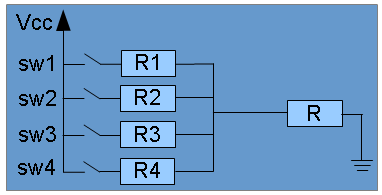
\includegraphics[width=12cm,scale=1]{resources/2_3-dipswitch.png}
	\caption{Diagrama de uno de los 3 divisores del dipswitch}
	\label{fig:\thefigure}
\end{figure}


\section{Firmware del updown} \label{sec:\thesection}
\subsection{Convenciones}
Con el objetivo de maximizar el encapsulamiento, las funciones dentro de los módulos se dividirán en internas y externas. Las internas podrán ser accedidas únicamente por otras funciones dentro del módulo, mientras que las externas también podrán ser accedidas por funciones de otros módulos.\\
En cuanto a variables, solo se utilizarán variables internas al módulo. En caso de poder ser accedidas externamente se hará a través de setters (devuelve el valor de la variable) y getters (escribe un valor en la variable).\\
Las funciones tendrán su nombre en formato \textit{camelCase} (priméra letra minúscula y el resto de las primeras letras de las palabras utilizadas en el nombre en mayúscula), los Define en \textit{MAYUSCULA}, y los módulos en formato PascalCase (como el camel case pero con la primera letra en mayúsucula).
Finalmente, todas las funciones y definiciones que pueden ser accedidas desde afuera de un módulo llevarán como prefijo el nombre del módulo seguido de un guión bajo. 

Además, debido a políticas de Blackout, todo el software desarrollado debe ser entendible por todo el equipo de trabajo. Esto quiere decir que una de las metas para las funciones de las librerías a crear es que permitan un flujo entendible, y que los nombres de las funciones sean parecidas a las de Arduino ya que lo que se acostumbraba a utilizar en la empresa para la programación de sistemas embebidos.\\
Para lograr este objetivo todas los módulos desarrollados tendrán una función de inicialización llamada "init", y de lectura y escritura, según corresponda, llamadas "read" y "write", respectivamente. 

A contunuación se presentan algunos ejemplos. Función de inicialización del módulo 1: Modulo1\_init(); Define del largo de un buffer genérido del modulo 3: Modulo3\_BUFFERGENERICO.


\subsection{Librerías de bajo nivel}
Como se mencionó en la sección \ref{sec:2.2}, se desarrollarán librerías para manejar los periféricos del Atmega328p y asi poder controlar el hardware del sistema.\\
Asociadas a las librerías viene de la mano el concepto de módulo, que tiene que ver con agrupar funciones similares en un mismo paquete para desacoplar dependencias y separar al sistema en varios subsistemas que sean lo más independientes que se pueda. Esto ayuda a que el programa sea escalable y mantenible, por lo que todo el software desarrollado se hará de manera modular.

Entonces, para manejar los periféricos se creará una librería de bajo nivel que constará de los siguientes módulos:
\begin{itemize}
	\item \textbf{Entradas y salidas digitales}, para leer el estado del fin de carrera y comandar el freno y los leds indicadores interno y externo. Este módulo se llamará \textit{DigitalIO}.
	\item \textbf{Entradas analógicas}, para leer las 3 salidas analógicas del dipswitch y poder determinar la posición de los selectores. Este módulo se llamará \textit{ADC}, por \textit{Analog to Digital Converter}.
	\item \textbf{Interrupciones externas} por cambio de estado de un pin, para llevar cuenta de los cambios de estado de los encoders AB y así saber la posición relativa. Este módulo se llamará \textit{EXINT}, por \textit{EXternal INTerrupts}.
	\item \textbf{PWM}, para el manejo del motor de continua. Este módulo se llamará \textit{PWM}, por \textit{Pulse Width Modulation}.
	\item \textbf{UART}, para la lectura de la señal DMX. Este módulo se llamará \textit{UART}, por \textit{Universal Asynchronous Receiver/Transmitter}
	\item \textbf{UART por software}, una UART implementada en pines genéricos que se utilizará para el debuggeo de la placa. Este módulo se llamará \textit{SUART}, por \textit{Software UART}.
	\item \textbf{Base de tiempo}, un timer utilizado para la temporización tareas y eventos. Este módulo se llamará \textit{Tick}.
\end{itemize}

\subsection{Librerías de alto nivel}
Hay que tener en cuenta que no es lo mismo obtener un valor analógico leyendo un registro del microcontrolador, que determinar qué conmutadores del dipswitch están activados leyendo 3 valores analógicos. Por lo tanto, se necesita una librería que sea más abstracata que la del manejo de periféricos para poder utilizar el hardware de esta aplicación en particular.\\
Entonces, se creará una librería propia de la aplicación que constará de los siguientes módulos:
\begin{itemize}
	\item \textbf{Dipswitch}, que incluye la lectura de las llaves del dipswitch, y la escritura del led indicador externo.
	\item \textbf{Grua}, que incluye el manejo del motor, del led interno, del freno y del fin de carrera.
	\item \textbf{DMX}, para la recepción de datos de la consola DMX.
	\item \textbf{Encoder}, para el manejo de los encoders AB del disco y del motor.
	\item \textbf{Controlador}, para la implementación del sistema de control
\end{itemize}

\newpage
\subsection{Diagrama de módulos}
De estas 2 librerías se obtiene el diagrama de módulos presentado en la figura \ref{fig:2.4}, el cual muestra su relación, dependencia y alcance. 

\begin{figure}[!ht]
	\centering
	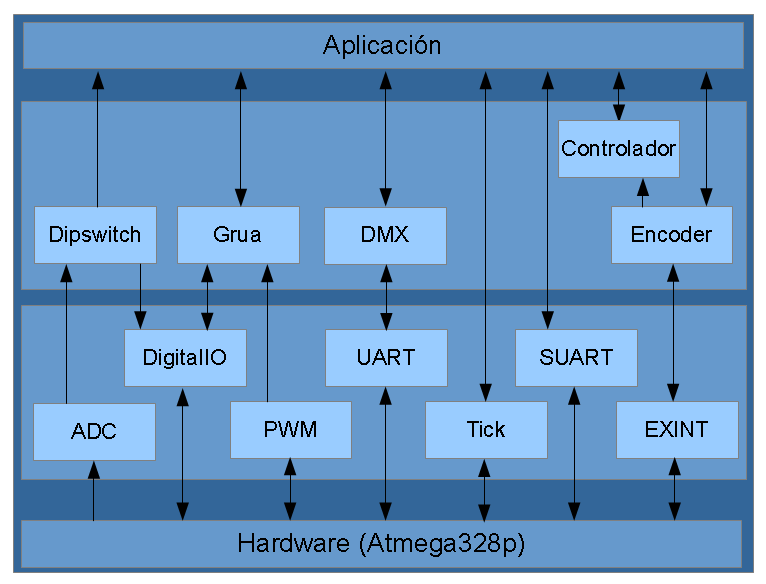
\includegraphics[width=14cm,scale=1]{resources/2_4-diagramaDeModulos.png}
	\caption{Diagrama de módulos del firmware}
	\label{fig:\thefigure}
\end{figure}
